\chapter{Introdução}
\label{chapter:introdcao}

\section{Contexto}

% Falar sobre sistemas de exaustão com exemplos
Sistemas de exaustão hoje em dia possuem uma forte colaboração na composição de sons e ruídos. Escapamentos, sistemas de ventilação, buzinas e motores aeronáuticos são exemplos desses sistemas que estão altamente presentes no dia-dia. Cada vez mais a sociedade vem desenvolvendo consciência crítica dos danos que os ruídos desses tipos de sistemas podem acarretar a saúde da população. Tal fato é tão preponderante que, como é apresentado por \citeonline{munjal}, desde os anos da década de 1920 há registros de esforços para entender e caracterizar esses tipos sistemas afim de colaborar com a manutenção e desenvolvimento de ambientes saudáveis no contexto acústico.

% Falar sobre dutos
Há vários elementos estruturais que podem compor sistemas de exaustão, mas os dutos circulares se caracterizam como fundamentais e bastante presentes. Sua forma cilíndrica permite que vários fenômenos físicos possam ocorrer e interagir entre si, principalmente os fenômenos acústicos e de fluxo de massa (escoamentos). De acordo com \citeonline{munjal}, o corpo de estudos e conhecimentos da acústica interna de dutos está bem estabelecido, mas verifica-se na literatura vários questionamentos sobre o funcionamento do mesmo na presença de escoamentos (fenômenos aeroacústicos). Em vista disso, determinar a caracterização da acústica interna de dutos é de extrema importância visto as várias tecnologias relacionadas a sistemas de exaustão sem um amparo técnico bem estabelecido da literatura no ponto de vista da aeroacústica.

% Falar sobre coeficiente de reflexão e correção comprimento
Em geral, pode-se utilizar dois parâmetros para caracterizar o fenômeno da acústica interna de dutos:

\begin{itemize}
    \item a magnitude do coeficiente de reflexão $\|R\|$, razão entre as componentes refletida e incidente da onda no duto, a qual é dada por
    \begin{equation}
        R_{r} =\frac{Z_{r} - Z_{0}}{Z_{r} + Z_{0}},
        \label{eq:R}
    \end{equation}
    sendo $Z_{r}$ a impedância de radiação e $Z_{0}$ a impedância característica do meio;
    
    \item coeficiente de correção da terminação normalizado pelo raio do duto $l/a$ em que $a$ é o raio do duto. Tal parâmetro representa o comprimento acústico efetivo do duto. Em outras palavras, o fator $l$ é a quantidade adicional medida a partir da abertura do duto a qual deve propagar a onda incidente antes de ser refletida para o interior do duto com fase invertida. Tal coeficiente de correção da terminação $l$ é dado por
    \begin{equation}
        l = \frac{1}{k} \arctan\!\left(\frac{Z_{r}}{Z_{0} \, \mathrm{i}}\right)
        \label{eq:l}
    \end{equation}
    sendo $k$ o número de onda.
\end{itemize}

Com o uso desses dois parâmetros pode-se projetar dutos com um comportamento acústico adequado a diversas situações que exigem atenuação de ruídos em certas frequências, além de poder prever com mais acurácia já que grande parte dos estudos consideram a acústica interna de dutos sem escoamentos.

\section{Problema}

Com relação ao contexto abordado, a solução exata para o problema de um duto circular não flangeado na ausência de escoamento foi proposta por \citeonline{levine1948radiation}. A solução assume que a espessura das paredes do duto são desprezíveis e o fluido é inviscido. A partir destas simplificações, as expressões exatas para $\|R\|$ e $l$ são obtidas utilizando-se a técnica de Wiener-Hopf.

Apesar da utilidade do modelo de Levine e Schwinger, em boa parte das aplicações práticas, dutos circulares transportam escoamentos médios. Para tais circunstâncias, \citeonline{munt1990acoustic} propôs um modelo analítico exato, também baseado na técnica de Wiener-Hopf, em que se considera a presença de um escoamento subsônico no interior do duto. Considera-se nesse modelo as premissas de que o escoamento é uniforme, invíscido e que a camada cisalhante do jato é infinitamente fina. Além disso, o modelo considera a condição de Kutta na borda do duto para lidar com a singularidade da velocidade de partícula nesta região.

É importante ressaltar que modelos exatos para os parâmetros de radiação de dutos se limitam às condições geométricas simples. No entanto, observa-se na prática terminações cujas geometrias divergem significativamente daquela associadas a um duto não flangeado. Exemplos comuns destas geometrias são aquelas encontradas em difusores, chaminés, sistemas de exaustão, $nozzles$ e instrumentos musicais. A Figura \ref{fig:diferentes_dutos} ilustra casos mais realistas de terminação de dutos comumente encontrados na prática. Para estes casos, não existem modelos que considerem a influência do escoamento nas propriedades de radiação. Além disso, a análise numérica considerando os efeitos de escoamento não é trivial.

No entanto, com o advento de novas tecnologias computacionais, é possível realizar procedimentos numéricos extremamente complexos com certa agilidade e precisão. $Softwares$ como \citeonline{ansys} e \citeonline{comsol} possuem a viabilidade de realizar cálculos de fluido dinâmica computacional de sistemas complexos como carros e aviões. Essa capacidade técnica é oriunda em maior parte pelas tecnologias de processamento paralelo multinúcleo de processadores e implementações de seus respectivos $softwares$ gerenciadores como Open MPI \citeonline{openmpi}. Essa evolução tecnológica vem sendo essencial para o surgimento de novas ferramentas para a exploração e descoberta de fenômenos físicos, antes muitas vezes inviáveis de estudar por alto custo de bancadas experimentais ou alta complexidade na consolidação de um modelo matemático representativo.  


\section{Objetivos}

Considerando a problemática discutida acima, o objetivo principal desse trabalho é desenvolver uma ferramenta computacional para análise do comportamento acústico interno de dutos com diferentes condições de contorno na presença de escoamentos de baixo número de Mach (M $<$ 0,2).

Tem-se como objetivos específicos:
\begin{itemize}
    \item modelar e analisar o comportamento acústico de dutos não flangeados sem escoamento;
    \item modelar e analisar o comportamento acústico de dutos não flangeados com escoamento de saída;
    \item modelar e analisar o comportamento de dutos terminados por difusores do tipo corneta cilíndrica com diferentes raios e escoamento de saída;
    \item modelar e analisar o comportamento acústico interno de dutos com escoamento sugado e diferentes geometrias de terminação.
\end{itemize}

\begin{figure}[ht!]
\centering
  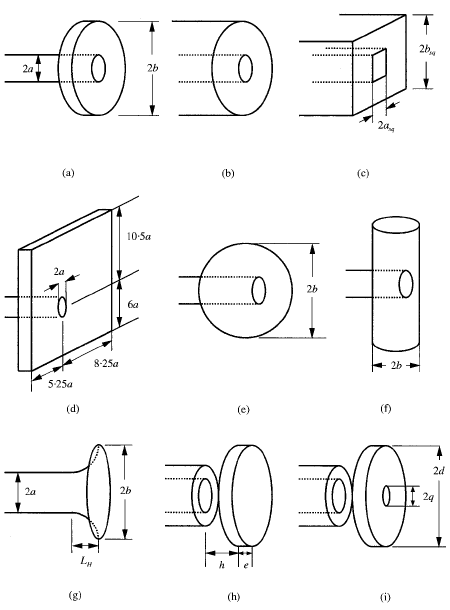
\includegraphics[width=.8\linewidth]{figuras/diferentes_dutos.png}
  \\
  \text{Fonte: \cite{dalmont2001radiation}}
  \captionof{figure}[Exemplos de várias termiações de dutos circulres.]{Exemplos de vários tipos de terminações: (a) flange circular; (b) flange circular com espessura do duto; (c) duto quadrado com flange de espessura quadrada; (d) flange normalizada; (e) flange esférica; (f) flange cilíndrica; (g) corneta; (h) disco não perfurado; (i) disco perfurado.}
  \label{fig:diferentes_dutos}
\end{figure}